\section{Introduction}
The main goal of this laboratory assignment is to analyse and better understand how AC/DC converters work and to find an optimal solution for the circuit built (i.e., a solution that allow one to get the result wanted at a minimal cost - having in mind that components like capacitors and resistors are very expensive comparatively with components like diodes).\\

AC/DC converters are circuits that act as transformers of the circuit's current from an alternating input (AC) - in this case of $230V$ and a frequency of $50Hz$ - to a direct output (DC) - which in the case will be of $12V$. \\

Essentially, these converters use rectifiers (which will turn the AC input into DC output - can be full-wave and half-wave as it will be seen), voltage regulators (that can limit positive and/or negative voltages and are made up of multiple diodes) and a reservoir capacitor which smooths the pulsating DC current.\\

The circuit used to simulate this was:

\begin{figure}[H]
    \centering
    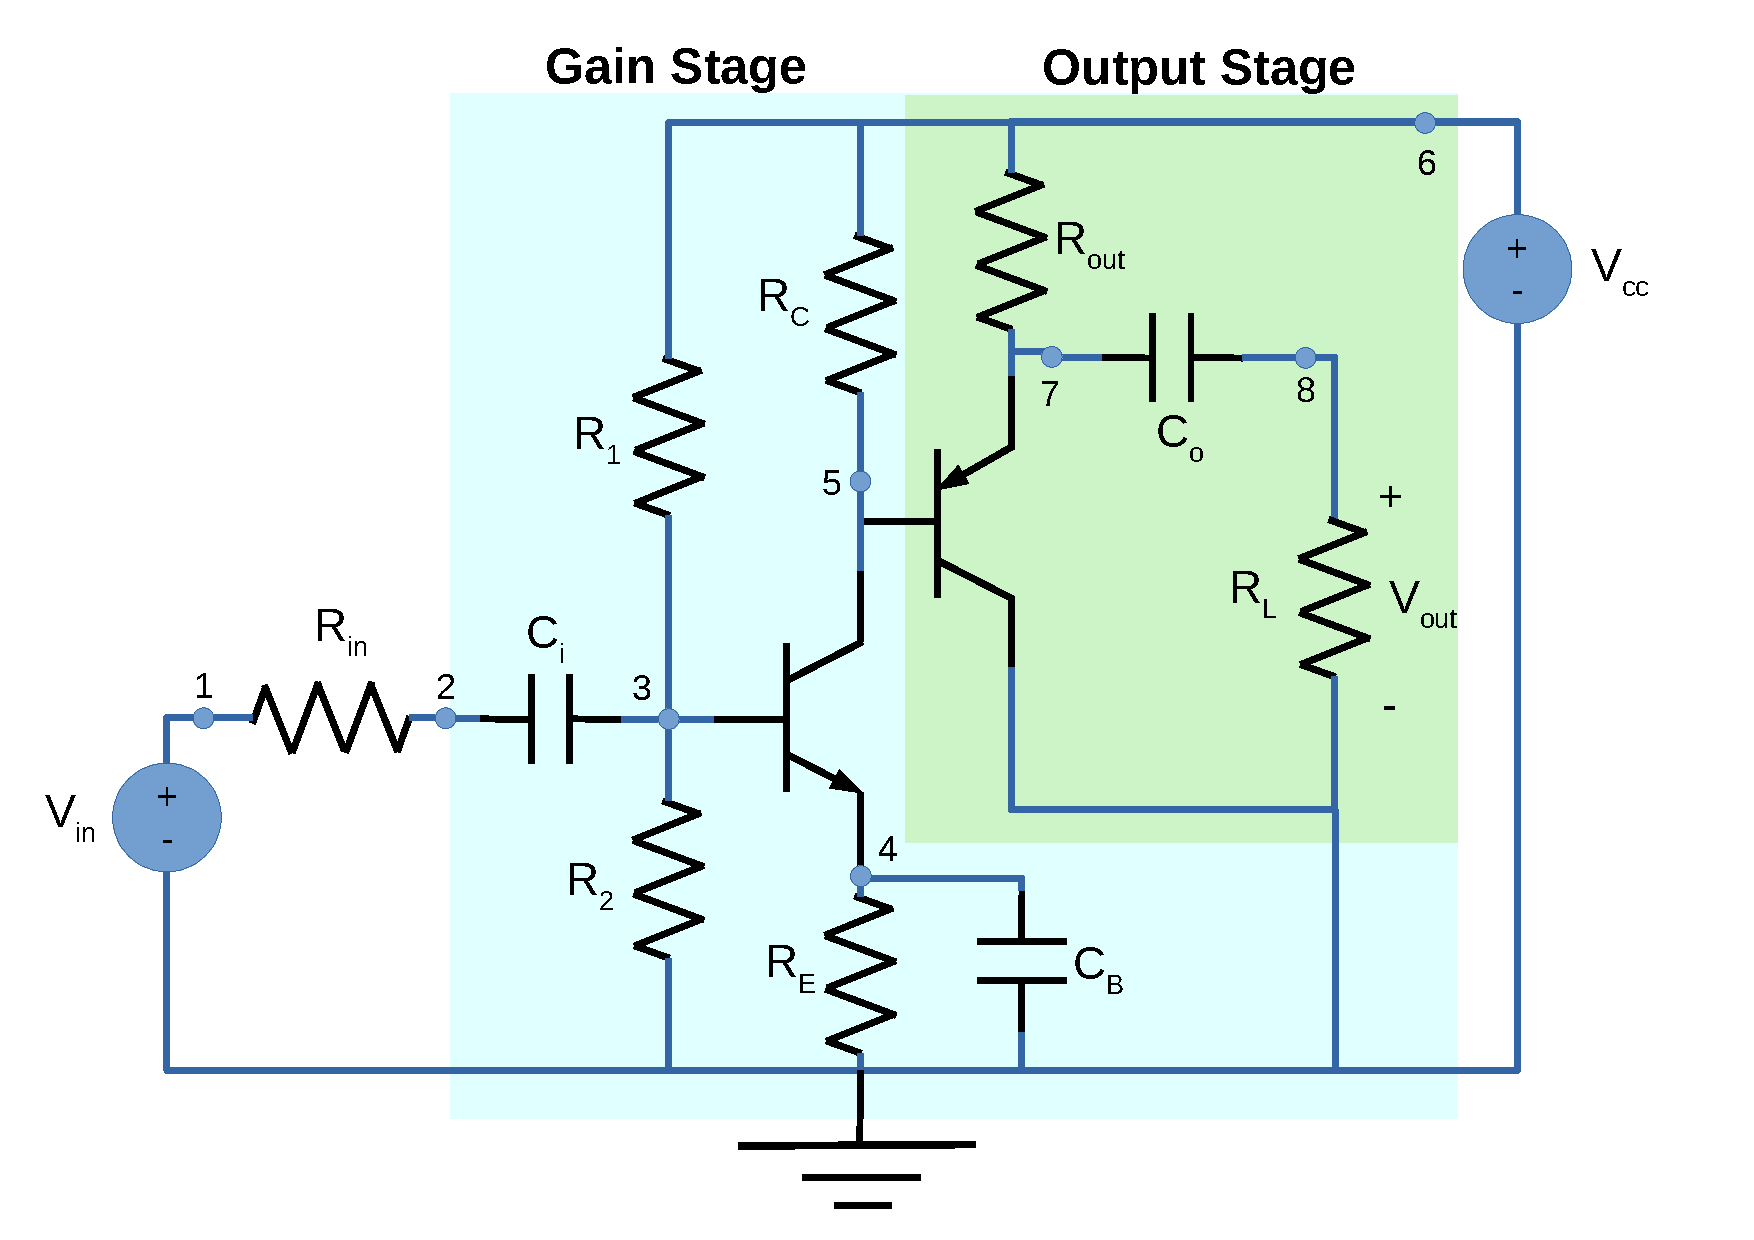
\includegraphics[width = 0.85\linewidth]{scheme.pdf}
            \caption{\textit{Circuit analysed. For the voltage dependent voltage source, one used $n = 17.78988$ - although this is not an integer, the students were motivated to use rational numbers for n.}}
    \label{fig:bigscheme}
\end{figure}

The results were obtained through a theoretical analysis, in which one predicted the output by using a theoretical method that suited the real circuit and through a simulation that was made using \textit{Ngspice}. The results obtained through both methods will be analysed throughout the report.\\

To evaluate the built circuit, one used a merit score which depended on the cost of the circuit, the output voltage ripples and the distance from the average value of output voltage obtained to the desired value ($V = 12V$). Then, as the AC/DC converter is as efficient as lower the cost, the ripples and the difference to the desired value are, the formula used to evaluate the score obtained with the AC/DC converter was:

\begin{equation}
    M = \frac{1}{c(r + d + 10^{-6})}
    \label{score}
\end{equation}

in which $c$ represents the total cost of the circuit, $r$ represents the output voltage ripples and $d$ represents the average value for $|v_0 - 12|$ in which $v_o$ is the output voltage.\\

To calculate the cost, one considered that the cost of the circuit equals the sum of the cost of the resistors, capacitors and diodes and the "price table" for this components is given as:

\begin{table}[H]
    \centering
    \begin{tabular}{c|c}
        \textbf{Component} &  \textbf{Price}\\
        \hline
        Resistors & 1 MU $k\Omega^{-1}$ \\
        Capacitors & 1 MU $\mu F^{-1}$ \\
        Diodes & 0.1 MU diode$^{-1}$
    \end{tabular}
    \caption{Price table for the components used}
    \label{tab:my_label}
\end{table}